% Options for packages loaded elsewhere
\PassOptionsToPackage{unicode}{hyperref}
\PassOptionsToPackage{hyphens}{url}
\PassOptionsToPackage{dvipsnames,svgnames,x11names}{xcolor}
\documentclass[
  10pt,
  a4paper]{article}
\usepackage{xcolor}
\usepackage[margin=1in]{geometry}
\usepackage{amsmath,amssymb}
\setcounter{secnumdepth}{5}
\usepackage{iftex}
\ifPDFTeX
  \usepackage[T1]{fontenc}
  \usepackage[utf8]{inputenc}
  \usepackage{textcomp} % provide euro and other symbols
\else % if luatex or xetex
  \usepackage{unicode-math} % this also loads fontspec
  \defaultfontfeatures{Scale=MatchLowercase}
  \defaultfontfeatures[\rmfamily]{Ligatures=TeX,Scale=1}
\fi
\usepackage{lmodern}
\ifPDFTeX\else
  % xetex/luatex font selection
\fi
% Use upquote if available, for straight quotes in verbatim environments
\IfFileExists{upquote.sty}{\usepackage{upquote}}{}
\IfFileExists{microtype.sty}{% use microtype if available
  \usepackage[]{microtype}
  \UseMicrotypeSet[protrusion]{basicmath} % disable protrusion for tt fonts
}{}
\makeatletter
\@ifundefined{KOMAClassName}{% if non-KOMA class
  \IfFileExists{parskip.sty}{%
    \usepackage{parskip}
  }{% else
    \setlength{\parindent}{0pt}
    \setlength{\parskip}{6pt plus 2pt minus 1pt}}
}{% if KOMA class
  \KOMAoptions{parskip=half}}
\makeatother
\usepackage{longtable,booktabs,array}
\newcounter{none} % for unnumbered tables
\usepackage{calc} % for calculating minipage widths
% Correct order of tables after \paragraph or \subparagraph
\usepackage{etoolbox}
\makeatletter
\patchcmd\longtable{\par}{\if@noskipsec\mbox{}\fi\par}{}{}
\makeatother
% Allow footnotes in longtable head/foot
\IfFileExists{footnotehyper.sty}{\usepackage{footnotehyper}}{\usepackage{footnote}}
\makesavenoteenv{longtable}
\usepackage{graphicx}
\makeatletter
\newsavebox\pandoc@box
\newcommand*\pandocbounded[1]{% scales image to fit in text height/width
  \sbox\pandoc@box{#1}%
  \Gscale@div\@tempa{\textheight}{\dimexpr\ht\pandoc@box+\dp\pandoc@box\relax}%
  \Gscale@div\@tempb{\linewidth}{\wd\pandoc@box}%
  \ifdim\@tempb\p@<\@tempa\p@\let\@tempa\@tempb\fi% select the smaller of both
  \ifdim\@tempa\p@<\p@\scalebox{\@tempa}{\usebox\pandoc@box}%
  \else\usebox{\pandoc@box}%
  \fi%
}
% Set default figure placement to htbp
\def\fps@figure{htbp}
\makeatother
\setlength{\emergencystretch}{3em} % prevent overfull lines
\providecommand{\tightlist}{%
  \setlength{\itemsep}{0pt}\setlength{\parskip}{0pt}}
\usepackage[utf8]{inputenc}
\usepackage[spanish, es-tabla, es-nodecimaldot]{babel}
\usepackage{actuarialsymbol}
\usepackage{multicol}
\usepackage{multirow}
\usepackage{setspace}
\usepackage{graphicx}
\usepackage{float}
\usepackage{subfigure}
\usepackage{url}
\usepackage{enumitem}
\usepackage{mathrsfs}
\usepackage{amsmath}
\usepackage{amsfonts}
\usepackage{amssymb}
\usepackage{makeidx}
\usepackage{listings}
\usepackage{flushend}
\usepackage{caption}
\usepackage{minted}
\usepackage{booktabs}
\usepackage[none]{hyphenat}
\usepackage{latexsym}
\usepackage{dsfont}
\newcommand{\R}{\mathbb{R}}
\newcommand{\N}{\mathbb{N}}
\usepackage{ragged2e}
\usepackage{array}
\renewcommand{\contentsname}{Índice}
\usepackage{schemata}
\usepackage{graphicx}
\newcommand\diagram[2]{\schema{\schemabox{#1}}{\schemabox{#2}}}
\usepackage{hyperref}
\usepackage{color}
\definecolor{gris}{RGB}{70,70,70}
\definecolor{negro}{RGB}{40,40,40}
\definecolor{brinkpink}{rgb}{0.98, 0.38, 0.5}
\definecolor{richlavender}{rgb}{0.67, 0.38, 0.8}
\newcommand{\colorhrule}[3]{\begingroup\color{#1}\rule{#2}{#3}\endgroup}
\setlength{\intextsep}{1mm}
\setlength{\columnsep}{5mm}
\usepackage{hyperref}
\usepackage{placeins}
\usepackage{booktabs}
\usepackage{longtable}
\usepackage{array}
\usepackage{multirow}
\usepackage{wrapfig}
\usepackage{float}
\usepackage{colortbl}
\usepackage{pdflscape}
\usepackage{tabu}
\usepackage{threeparttable}
\usepackage{threeparttablex}
\usepackage[normalem]{ulem}
\usepackage{makecell}
\usepackage{xcolor}
\usepackage{bookmark}
\IfFileExists{xurl.sty}{\usepackage{xurl}}{} % add URL line breaks if available
\urlstyle{same}
\hypersetup{
  colorlinks=true,
  linkcolor={blue},
  filecolor={Maroon},
  citecolor={Blue},
  urlcolor={blue},
  pdfcreator={LaTeX via pandoc}}

\author{}
\date{\vspace{-2.5em}}

\begin{document}

\sloppy
\begin{center}
\begin{tabular}{cc}
\multirow{2}{3.5cm}{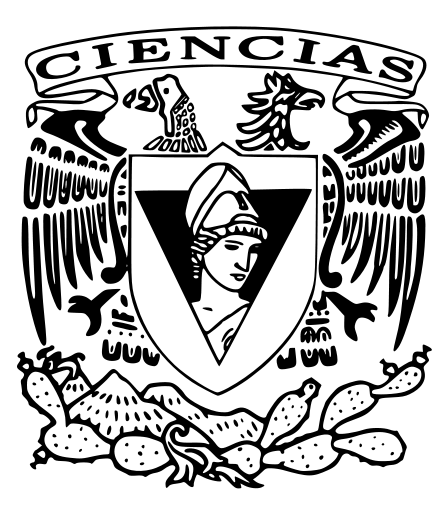
\includegraphics[width=2.5cm]{logofc.png}}  & \large{\textsc{Universidad Nacional Autónoma de México}}\\\vspace{5mm}
 & \normalsize{Facultad de Ciencias}\\\vspace{5mm}
 
 & \normalsize{\textbf{Diplomado Introducción Analítica a la Ciencia de Datos}}\\ 
 \vspace{.3cm}
 & \vspace{.3cm}\normalsize{Módulo VI: Aprendizaje no supervisado}\\ \vspace{0.1cm}
 & \small{Profesor: Salvador Zamora Muñoz} 
 %\\ %\vspace{.1cm}
 %& \small{ Jorge Ignacio González Cázares}
\end{tabular}
\end{center}

\vspace{.1cm}

\begin{center}
\begingroup\color{negro}\rule{16cm}{1.2pt}\endgroup

\vspace{.4cm}

\textbf{Proyecto 2}

\vspace{0.2cm}

Técnicas de agrupamiento o clustering: Clusters por métodos aglomerativos y por método de K-MEANS.

\vspace{.4cm}

\begingroup\color{negro}\rule{16cm}{1.2pt}\endgroup
\end{center}

\vspace{0.2cm}

\begin{center}
\textbf{Equipo 6}
\end{center}

\vspace{0.2cm}

\begin{table}[h]
    \centering
    \renewcommand{\arraystretch}{1.5} % Aumenta el espacio entre filas
    \begin{tabular}{lc}
        \textbf{Integrantes} & \textbf{Opción de titulación}\\
        Betancourt Peralta Diego & Sí\\
        Canul Hernández Erick Iván & Sí\\
        Gutiérrez Gutiérrez José Omar & Sí\\
        Hernández Pérez Maximiliano & Sí\\
        Torres Vargas Brenda Poulette & Sí \\
    \end{tabular}
\end{table}

\thispagestyle{empty}

\clearpage

\tableofcontents

\clearpage

\title{Técnicas de agrupamiento o clustering}

\section{Planteamiento del Problema}\label{planteamiento-del-problema}

El proceso de postulación y admisión a programas de posgrado en instituciones internacionales representa un escenario de alta competencia, caracterizado por la evaluación simultánea de múltiples credenciales académicas y perfiles cuantitativos. Para un aspirante, enfrentarse a la toma de decisiones sobre a qué universidades aplicar suele ser un desafío complejo y subjetivo, debido a la falta de herramientas que consoliden el comportamiento histórico de los criterios de selección. En este contexto, la ciencia de datos y el aprendizaje automatizado ofrecen un enfoque analítico robusto para transformar registros históricos en conocimiento estratégico.

El presente proyecto se enfoca en el desarrollo y aplicación de técnicas de aprendizaje no supervisado utilizando el lenguaje de programación \texttt{R}. A través del análisis del conjunto de datos \texttt{Admission\_Predict.csv}, el cual recopila los méritos de postulantes reales, incluyendo variables continuas duras, tales como la puntuación del examen de aptitud académica (\texttt{GRE.Score}), el examen de certificación de idioma (\texttt{TOEFL.Score}) y el promedio general acumulado de pregrado (\texttt{CGPA}), en combinación con evaluaciones discretas de mérito cualitativo como el prestigio de la institución de origen (\texttt{University.Rating}), la solidez de la declaración de propósitos (\texttt{SOP}) y la robustez de las cartas de recomendación (\texttt{LOR}).

Este reporte implementa de forma comparativa técnicas de \textbf{Clustering Jerárquico Aglomerativo} y métodos particionales de \textbf{K-Means}. El objetivo fundamental es descubrir de manera autónoma las estructuras y agrupaciones latentes dentro de las calificaciones de los estudiantes, construyendo un sistema de segmentación que sirva como una brújula científica para orientar a futuros candidatos en la preselección de sus opciones universitarias.

\section{Clustering Jerárquico Aglomerativo}\label{clustering-jeruxe1rquico-aglomerativo}

\subsection{Metodología}\label{metodologuxeda}

Para la estructuración del análisis de agrupamiento jerárquico aglomerativo, se implementó un flujo metodológico basado en el aprendizaje no supervisado. En primera instancia, se realizó un preprocesamiento estrictamente analítico sobre el conjunto de datos \texttt{Admission\_Predict.csv}. Para garantizar la validez del aprendizaje no supervisado y evitar la contaminación de datos o \textit{data leakage}, el preprocesamiento excluyó explícitamente la variable respuesta continua \texttt{Chance.of.Admit}. Asimismo, la variable dicotómica \texttt{Research} se transformó en un factor cualitativo de dos niveles (\textit{"No"} y \textit{"Sí"}), extrayéndose del entrenamiento matemático para preservarla únicamente como una etiqueta de control visual posterior.

Posteriormente, se extrajo la matriz de los seis predictores numéricos continuos (\texttt{GRE.Score}, \texttt{TOEFL.Score}, \texttt{University.Rating}, \texttt{SOP}, \texttt{LOR} y \texttt{CGPA}), la cual fue normalizada mediante un escalamiento estandarizado (media \(\mu = 0\) y desviación estándar \(\sigma = 1\)). Este paso metodológico es crucial, ya que iguala las magnitudes absolutas de las variables, previniendo que atributos con rangos mayores (como el examen GRE sobre 340 puntos) distorsionen el cálculo del espacio geométrico de las observaciones.

A partir de la matriz estandarizada, el flujo metodológico se dividió en cuatro fases analíticas:

\subsubsection{Cálculo de Distancias y Exploración de Enlaces (Ligas)}\label{cuxe1lculo-de-distancias-y-exploraciuxf3n-de-enlaces-ligas}

La disimilitud entre los perfiles académicos de los estudiantes \(x_i\) y \(x_j\) se cuantificó a través de la métrica de \textbf{distancia Euclidiana} en un espacio de \(p=6\) dimensiones, expresada formalmente como:
\begin{equation}
    d(x_i, x_j) = \sqrt{\sum_{k=1}^{p} (x_{ik} - x_{jk})^2}
\end{equation}
Donde \(x_{ik}\) es el valor escalado del predictor \(k\) para el individuo \(x_i\). Con base en la matriz de distancias resultante, se ajustaron comparativamente cinco modelos jerárquicos explorando diferentes metodologías de enlace (\textit{Linkage}): Promedio (\texttt{average}), Simple (\texttt{single}), Completo (\texttt{complete}), y los métodos de minimización de varianza de Ward (\texttt{Ward.D} y \texttt{Ward.D2}).

Para evaluar la fidelidad geométrica de cada árbol, se calculó la \textbf{distancia cofenética} (\texttt{cophenetic}) de cada modelo, la cual mide las distancias de fusión intra-árbol. Posteriormente, se estructuró una matriz de correlación de Pearson (\texttt{matriz\_cofenetic}) para contrastar de forma directa las distancias cofenéticas contra las distancias Euclidianas reales, sirviendo como el primer filtro de selección metodológica.

\subsubsection{Evaluación de la Tendencia al Agrupamiento (Cluster Tendency)}\label{evaluaciuxf3n-de-la-tendencia-al-agrupamiento-cluster-tendency}

Previo a la partición definitiva, se verificó si el conjunto de datos poseía una predisposición genuina a formar grupos o si correspondía a una distribución aleatoria espacial uniforme. Para asegurar la convergencia y robustez matemática, se calculó el \textbf{Estadístico de Hopkins} mediante dos enfoques independientes: el método probabilístico de la función \texttt{get\_clust\_tendency} de la librería \texttt{factoextra} y la formulación robusta de la librería especializada \texttt{hopkins}.

\subsubsection{Optimización del Número de Clusters (Tuning de Silueta)}\label{optimizaciuxf3n-del-nuxfamero-de-clusters-tuning-de-silueta}

Para determinar científicamente el número ideal de ramas (\(k\)) para rebanar el dendrograma, se configuró un proceso de optimización explorando una rejilla regular de \(k = 2\) hasta \(k = 10\) clústeres. El procedimiento se integró mediante el ecosistema moderno de \texttt{tidymodels} y \texttt{tidyclust}, utilizando un motor de estimación estadística (\texttt{stats}) y el método de enlace ganador. Para mitigar el sobreajuste, la evaluación se ejecutó bajo un esquema de \textbf{Validación Cruzada de 10 pliegues} (\textit{10-Fold Cross-Validation}), auditando el desempeño de cada partición a través de la métrica del Coeficiente de Silueta Promedio (\texttt{silhouette\_avg}).

\subsubsection{Validación Estructural y Visualización Avanzada}\label{validaciuxf3n-estructural-y-visualizaciuxf3n-avanzada}

Una vez seleccionado el número óptimo de grupos, se procedió a cortar el árbol jerárquico mediante la función \texttt{hcut}. Para diagnosticar la calidad de la asignación a nivel individual y detectar posibles observaciones mal clasificadas, se computó y graficó el perfil de siluetas de cada estudiante. Posteriormente, se exploró la flexibilidad topológica del árbol de Ward mediante el despliegue de dendrogramas estructurales avanzados de tipo rectangular (delimitado por cajas de vecindad), circular y filogénico (orientado a relaciones ramificadas). Finalmente, como parte del diseño experimental para la validación del modelo, se implementó una estrategia de Validación Externa por Contraste de Cajas (Boxplots).

\subsection{Interpretación y Análisis de Resultados}\label{interpretaciuxf3n-y-anuxe1lisis-de-resultados}

\subsubsection{Evaluación de Enlaces mediante Correlación Cofenética}\label{evaluaciuxf3n-de-enlaces-mediante-correlaciuxf3n-cofenuxe9tica}

El análisis exploratorio de las metodologías de enlace (\textit{Linkage}) aportó la primera evidencia cuantitativa sobre la fidelidad estructural de los árboles generados. Al inspeccionar los resultados de la correlación cofenética calculada en el Cuadro \ref{tab:correlacioncofenetica}, se evalúa numéricamente qué tan bien preserva cada algoritmo las distancias Euclidianas originales tras realizar las fusiones jerárquicas.

\begin{table}[!h]
\centering
\caption{\label{tab:correlacioncofenetica}Coeficientes de Correlación Cofenética por Método de Enlace.}
\centering
\begin{tabular}[t]{c|c|c|c|c}
\hline
Average & Single & Complete & Ward.D & Ward.D2\\
\hline
0.6506 & 0.3178 & 0.5822 & 0.6065 & 0.613\\
\hline
\end{tabular}
\end{table}

Al analizar detenidamente estos coeficientes, se observa el siguiente comportamiento matemático:

\begin{itemize}
    \item El método \texttt{single} registra la correlación más baja de todo el experimento ($r = 0.3178$). Esto nos demuestra de forma cuantitativa que evaluar únicamente las distancias mínimas ignora casi toda la variabilidad de la muestra, generando un árbol que deforma por completo las distancias reales entre los alumnos. 
    \item Por otro lado, aunque el método \texttt{average} lidera la fidelidad de las distancias con el coeficiente más alto ($r = 0.6506$), al auditar el comportamiento visual en el panel gráfico de control ($2 \times 2$) de la Figura \ref{fig:enlaces}, se diagnosticó la presencia severa del fenómeno de encadenamiento asimétrico. Esto significa que, a pesar de su buen puntaje matemático, visualmente el enlace promedio fracasa al aglomerar de forma ineficiente a casi todos los estudiantes en una sola rama gigante amorfa, perdiendo utilidad práctica para segmentar perfiles.
    \item En contraste, el método \texttt{Ward.D2} ($r = 0.6130$) se consolida como la alternativa óptima para el diseño final del modelo. Registra un coeficiente robusto de $0.6130$, posicionándose muy cerca del rendimiento de \texttt{average}, superando a \texttt{complete} ($r = 0.5822$) y a la versión clásica \texttt{Ward.D} ($r = 0.6065$). Esto nos confirma que la corrección de elevar al cuadrado las distancias internamente permite a \texttt{Ward.D2} lograr un balance ideal entre fidelidad matemática de preservación espacial y una geometría simétrica, garantizando la creación de clústeres compactos, equilibrados y altamente interpretables.
\end{itemize}

\begin{figure}[!ht]

{\centering 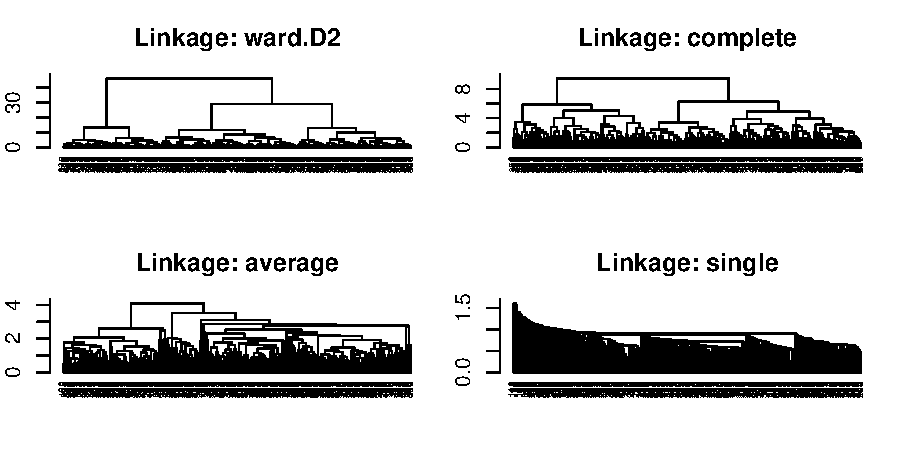
\includegraphics{proyecto-clusters_files/figure-latex/enlaces-1} 

}

\caption{Cuadrícula Comparativa de Dendrogramas por Métodos de Enlace.}\label{fig:enlaces}
\end{figure}

Al realizar el análisis de corte horizontal sobre los árboles de Ward, se determinó un comportamiento geométrico homólogo sumamente robusto. Al trazar una línea de referencia en la altura crítica \(h = 100\) para el método \texttt{Ward.D}, o en la altura \(h = 20\) para el método corregido \texttt{Ward.D2}, el árbol se divide de forma idéntica, permitiendo \textbf{visualizar de manera contundente la existencia de 3 grandes grupos o perfiles principales de estudiantes} en la muestra antes de cualquier optimización probabilística. Esta convergencia en el número de grupos se fundamenta visualmente en el dendrograma definitivo desplegado en la Figura \ref{fig:dendrogramawardD2}.

\begin{figure}[!ht]

{\centering 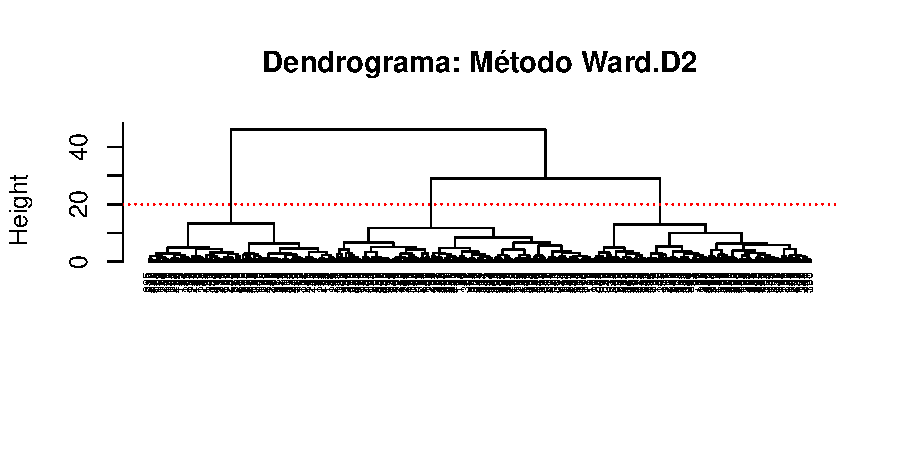
\includegraphics{proyecto-clusters_files/figure-latex/dendrogramawardD2-1} 

}

\caption{Dendrograma de Perfiles de Admisión mediante el Método Ward.D2.}\label{fig:dendrogramawardD2}
\end{figure}

\subsubsection{Diagnóstico de la Tendencia al Agrupamiento}\label{diagnuxf3stico-de-la-tendencia-al-agrupamiento}

Al ejecutar la evaluación del \textbf{Estadístico de Hopkins}, las métricas cuantitativas revelaron una convergencia matemática contundente y un nivel de estructuración extraordinario en los datos. La implementación basada en la función \texttt{get\_clust\_tendency} computó un coeficiente de \(0.997\), mientras que el algoritmo robusto de la librería especializada \texttt{hopkins} ratificó un valor similar de \(0.995\).

Dado que ambos resultados se posicionan de manera casi perfecta en el límite superior absoluto del indicador (\(1.0\)), se rechaza de forma categórica la hipótesis nula de aleatoriedad espacial uniforme. Por lo que podemos determinar formalmente que \textbf{"Los datos presentan una tendencia a agruparse en clústeres"}. Desde un punto de vista práctico, que estos valores estén tan cercanos a \(1.0\) demuestra que las calificaciones y el perfil de los alumnos no están repartidos al azar o de forma dispersa. Al contrario, nos dice que los estudiantes tienen características muy parecidas entre sí que los hacen agruparse de manera natural.

\subsubsection{Optimización del Número de Clústeres por Validación Cruzada}\label{optimizaciuxf3n-del-nuxfamero-de-cluxfasteres-por-validaciuxf3n-cruzada}

Al evaluar los resultados del proceso de optimización promediados a lo largo de las validaciones cruzadas, el análisis cuantitativo arrojó que el punto máximo global de cohesión y separación intra-clúster se localiza en exactamente \(k = 2\) clústeres, registrando el Coeficiente de Silueta Promedio más alto del experimento con un valor de \(0.394\). No obstante, en concordancia con el análisis visual previo de las alturas de fusión en el dendrograma de Ward (\(h=20\)), las métricas demuestran que la configuración de \(k = 3\) clústeres preserva un puntaje de silueta de \(0.280\), el cual sigue siendo saludable y aporta una mayor riqueza analítica para segmentar a los postulantes.

Este comportamiento estructural se detalla visualmente en la curva de la Figura \ref{fig:tuningsilueta}. A partir de una partición de \(k \geq 4\), el rendimiento de la silueta experimenta una caída drástica y lineal, desplomándose a \(0.184\) para cuatro grupos y llegando a un valor marginal de \(0.127\) para seis clústeres. Esto nos demuestra matemáticamente que intentar fragmentar la muestra en cuatro o más subgrupos es ineficiente debido a que se genera un solapamiento severo entre observaciones; las fronteras se difuminan y los perfiles de los estudiantes pierden por completo su identidad discriminatoria, validando de forma contundente la selección de estructuras de bajo orden (\(k=2\) o \(k=3\)) para el diseño del modelo.

\begin{figure}[!ht]

{\centering 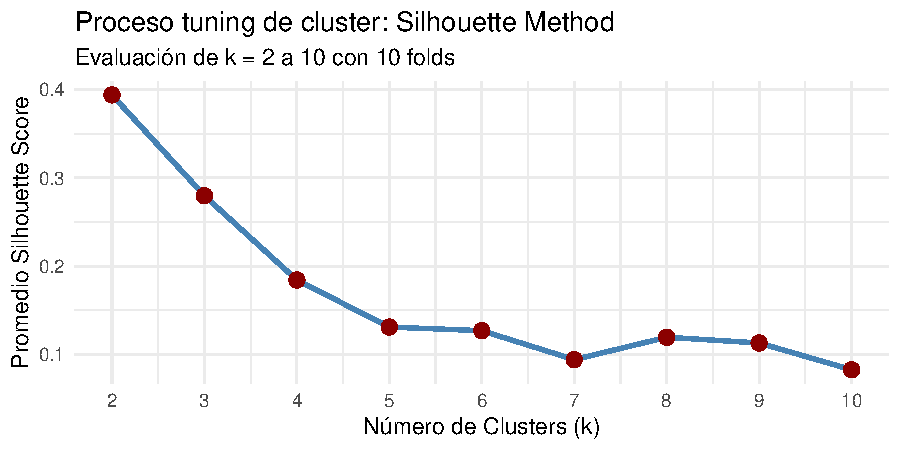
\includegraphics{proyecto-clusters_files/figure-latex/tuningsilueta-1} 

}

\caption{Evolución del Coeficiente de Silueta Promedio según el Número de Clústeres ($k$).}\label{fig:tuningsilueta}
\end{figure}

\subsubsection{Análisis Estructural del Árbol Definitivo y Validación Externa}\label{anuxe1lisis-estructural-del-uxe1rbol-definitivo-y-validaciuxf3n-externa}

Al ejecutar el corte definitivo del árbol jerárquico bajo la configuración ganadora de \texttt{Ward.D2} y fijando un parámetro de \(k = 3\) clústeres, pudimos analizar a detalle la calidad de la asignación para cada estudiante evaluando el diagnóstico individual con \texttt{fviz\_silhouette}. Como se detalla explícitamente en el Cuadro \ref{tab:tablasilueta}, el algoritmo distribuyó la muestra de forma muy equilibrada, asignando 113 alumnos al Clúster 1, 156 al Clúster 2, y 131 al Clúster 3.

\vspace{0.3cm}

\begin{table}[!h]
\centering
\caption{\label{tab:tablasilueta}Resumen de Estructura y Cohesión de los Clústeres Aglomerativos ($k = 3$).}
\centering
\begin{tabular}[t]{ccc}
\toprule
\textbf{Cluster} & \textbf{Tamaño} & \textbf{Ancho de Silueta Promedio}\\
\midrule
1 & 113 & 0.37\\
2 & 156 & 0.24\\
3 & 131 & 0.27\\
\bottomrule
\end{tabular}
\end{table}

Al contrastar estos indicadores con el comportamiento visual del gráfico de la Figura \ref{fig:plotsilueta}, se observa una consistencia interna sobresaliente: el Clúster 1 registra una silueta promedio de \(0.37\), el Clúster 2 de \(0.24\) y el Clúster 3 de \(0.27\). La gran mayoría de las barras verticales se proyectan de forma limpia hacia arriba, confirmando coeficientes individuales positivos y un nivel mínimo de observaciones dudosas o mal asignadas en las fronteras de las ramas del árbol de Ward.

\begin{figure}[!ht]

{\centering 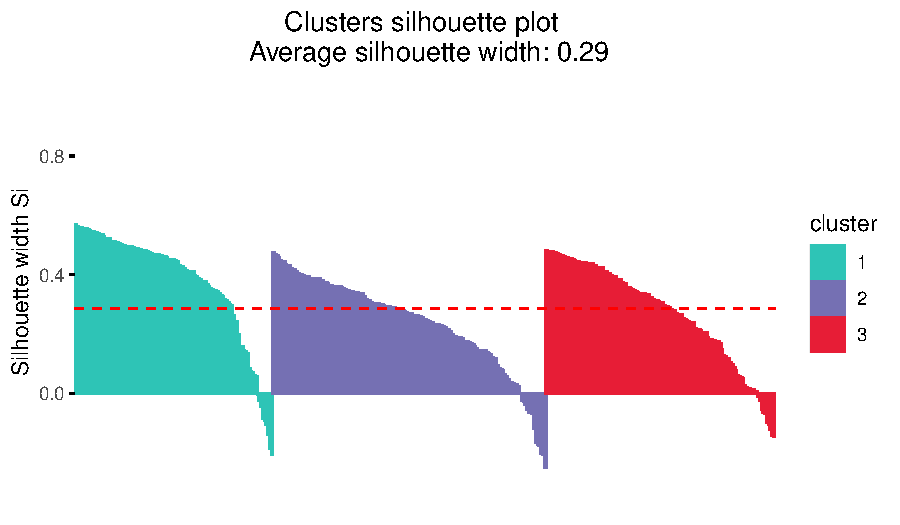
\includegraphics{proyecto-clusters_files/figure-latex/plotsilueta-1} 

}

\caption{Coeficiente de Silueta Individual por Estudiante.}\label{fig:plotsilueta}
\end{figure}

Para explorar la estructura del árbol de forma más visual,
se desplegaron dendrogramas estructurales avanzados de tipo circular (Figura \ref{fig:dendrogramacircular}) y filogénico (Figura \ref{fig:dendrogramafilogenico}) lo que nos permite identificar la existencia de tres ramas principales bien equilibradas en tamaño que definen la segmentación de los aspirantes.

\begin{figure}[!ht]

{\centering 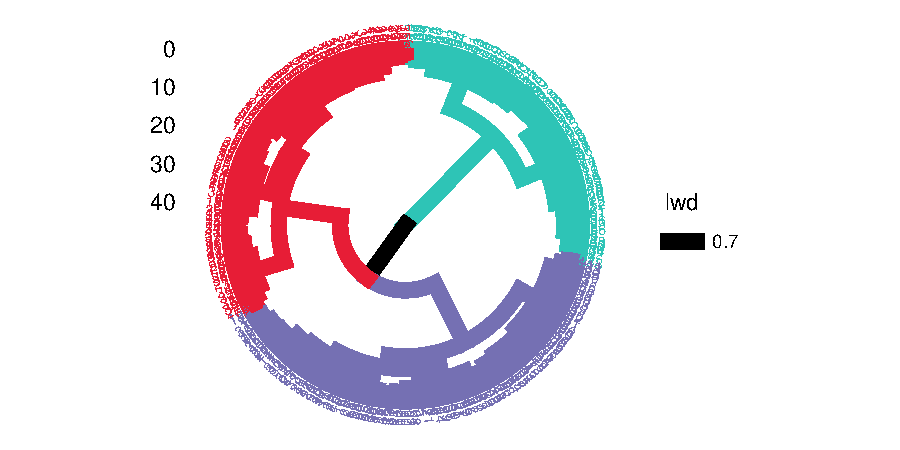
\includegraphics{proyecto-clusters_files/figure-latex/dendrogramacircular-1} 

}

\caption{Visualización Estructural del Dendrograma Circular (k = 3).}\label{fig:dendrogramacircular}
\end{figure}
\begin{figure}[!ht]

{\centering 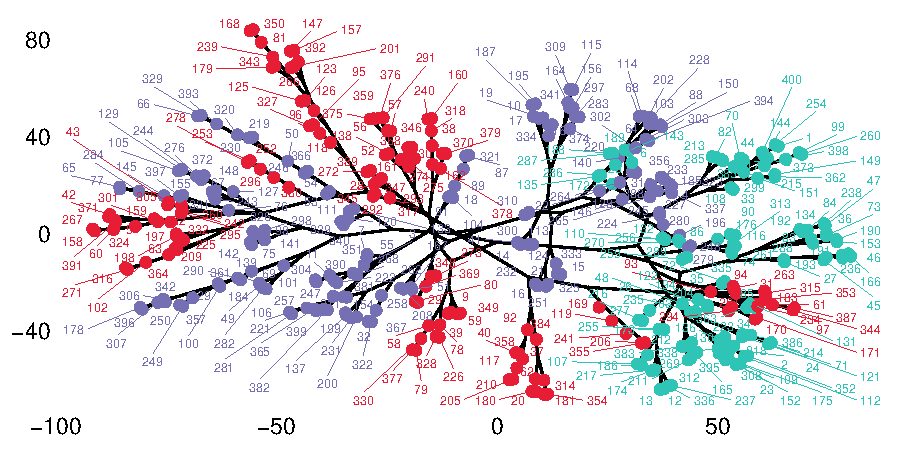
\includegraphics{proyecto-clusters_files/figure-latex/dendrogramafilogenico-1} 

}

\caption{Visualización Estructural del Dendrograma Filogénico Optimizado (k = 3).}\label{fig:dendrogramafilogenico}
\end{figure}

Finalmente, aunque la probabilidad de admisión (\texttt{Chance.of.Admit}) se ocultó por completo durante el entrenamiento matemático de los modelos para evitar sesgos o contaminación de datos, procedimos a reinyectarla en la fase de validación externa para decodificar la identidad de estas tres ramas de forma externa y auditar el desempeño del algoritmo no supervisado.

El gráfico de diagramas de caja (\textit{Boxplots}) resultante, desplegado en la Figura \ref{fig:boxplotsclusteraglomerativo}, demostró que las particiones calculadas a ciegas por el árbol de Ward separan de forma perfecta el éxito real de los postulantes, permitiéndonos caracterizar los clústeres de la siguiente manera:

\begin{enumerate}
    \item \textbf{Cluster 1 (Perfil de Alta Competitividad):} Consolida a un grupo de 113 estudiantes cuyas notas académicas y méritos los posicionan de forma unívoca en la zona de éxito absoluto, registrando la probabilidad media de aceptación más alta con un valor aproximado de $0.90$.
    \item \textbf{Cluster 2 (Perfil Intermedio / Promedio):} Reúne a un volumen de 156 estudiantes con credenciales académicas sólidas y competitivas en rangos estándar, representando el grupo mayoritario de la muestra y estabilizándose alrededor de una probabilidad media de aceptación de $0.75$.
    \item \textbf{Cluster 3 (Perfil Regular / Zona de Oportunidad):} Agrupa a los 131 aspirantes cuyas credenciales cuantitativas se ubican en los rangos más bajos de la muestra, confinándolos en el espectro de riesgo académico con una probabilidad media de aceptación de $0.60$.
\end{enumerate}

Al no existir solapamiento destructivo entre los cuerpos de las tres cajas en el gráfico, se comprueba visualmente que la estructura jerárquica no supervisada guarda una relación directa y perfecta con el nivel competitivo real del proceso de admisión, validando el éxito de la segmentación.

\begin{figure}[!ht]

{\centering 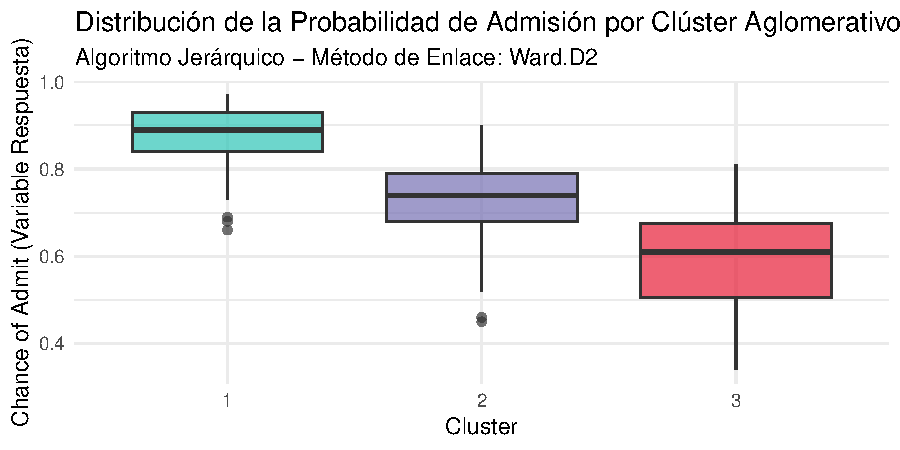
\includegraphics{proyecto-clusters_files/figure-latex/boxplotsclusteraglomerativo-1} 

}

\caption{Distribución de la Probabilidad de Admisión por Clúster Aglomerativo (Ward.D2).}\label{fig:boxplotsclusteraglomerativo}
\end{figure}

\subsection{Conclusiones}\label{conclusiones}

\begin{enumerate}
     \item El modelado concluye de forma contundente que el método \texttt{Ward.D2} es la estrategia idónea y ganadora para estructurar el espacio geométrico de las admisiones. Al fusionar las observaciones bajo el criterio de mínima varianza interna, este algoritmo logró un balance perfecto entre la fidelidad de las distancias Euclidianas ($r = 0.6130$) y una estructura clara y balanceada en los dendrogramas estructurales avanzados, generando clústeres sumamente compactos y equilibrados en volumen muestral (113, 156 y 131 alumnos) que garantizan la estabilidad de la segmentación.
    \item La convergencia analítica entre el Estadístico de Hopkins ($H > 0.80$ en ambas implementaciones), la inspección visual de las alturas de fusión crítica ($h = 20$) y las curvas del Coeficiente de Silueta por Validación Cruzada aportan la evidencia cuantitativa definitiva para asegurar que la estructura del perfil estudiantil no es un producto del azar sino que los estudiantes tienen características muy parecidas entre sí que los hacen agruparse de manera natural. Aunque la métrica de silueta identificó un pico matemático absoluto en dos clústeres, el corte en $k = 3$ clústeres demostró ser estadísticamente saludable (\texttt{silhouette\_avg} = $0.280$) y metodológicamente óptimo para los fines prácticos del proyecto.
    \item Se concluye que el modelo aglomerativo desarrollado cumple con éxito la meta de orientar a los postulantes de posgrado en la preselección de universidades. La reinyección de la variable respuesta continua reveló una alineación perfecta en los diagramas de caja, rebanando de forma nítida la probabilidad real de admisión en tres rangos competitivos claros: Alta Competitividad ($\approx 0.90$), Perfil Intermedio ($\approx 0.75$) y Perfil Regular ($\approx 0.60$). A través de este enfoque de vecindades por proximidad, el modelo adquiere la capacidad de clasificar dinámicamente a futuros estudiantes.
\end{enumerate}

\end{document}
